% Add something like "Its important to know how a browser loads a webpage?
Both browsers and mobile applications typically load content using the HTTP(S) protocol. When a user directs the browser (or application) to a new URL, the browser's Object Loader fetches the root HTML object, as depicted
in Figure~\ref{fig:network-diagram}. The HTML Parser launches additional
fetch requests for each linked resource within the HTML. In this way, the browser incrementally generates the DOM.
As the page loads, the Rendering component paints the UI.

From the user's perspective, the performance of a website can be defined according to a number of different metrics~\cite{above-the-fold,speed-index}. Here,
we focus on page load time, which is simple to measure
and loosely standardized across browsers~\cite{w3c-onload}.

\textbf{Page Load Time}. Roughly speaking, page load time (PLT) is the elapsed time from the moment a user requests a web page to the moment all resources on the page have been loaded~\cite{page-speed}.
We measure PLT by listening to the browser's Javascript \texttt{onload} event,
which fires in most browsers when all resources have been added to the DOM, and all images,
scripts, links, and sub-frames have finished loading~\cite{w3c-onload}.

%\colin{Need to make clear that certain objects (tasks) are dependent on others. When a task is dependent on another, it must wait until its dependencies (tasks) have completed. E.g., all tasks are dependent on the HTML parsing task for the root HTML)}
%\jamshed{Added this to "Critical Path" section


\textbf{Critical Path}. Web pages are comprised of many objects, such as images, Javascript, CSS, and HTML.
Each of these objects is handled by multiple (possibly concurrent) browser tasks: it must be
fetched, parsed or evaluated, and rendered. We refer to the non-overlapping
delays involved in parsing and rendering an object as its `computational
delay,' and refer to the fetch delay as its `network delay.'

Critical path analysis is a method for analyzing the performance of parallel
processes such as browsers.
Certain load tasks are dependent on others and must wait until their
predecessor tasks have completed. The critical path of a web page is the longest chain of dependent browser tasks such that reducing the length of any task not on the critical
path will not change the page load time~\cite{sarkar1987partitioning}.
In Figure~\ref{fig:plt-diagram}, the network and computational delay for the HTML, CSS, JS, and JPEG
objects determine the PLT. If we were to decrease the delay for loading the
PNG object, the critical path would remain the same, and therefore, the PLT would not change.

%\colin{Should make a clearer definition for `tasks' and `objects'. The web page is composed of multiple objects, each of which must be fetched (1 task), parsed or evaluated (1 task), and rendered (1 task).}

% TODO(cs): say whether it's possible that objects on the critical path can
% overlap or not. I think it is possible, e.g., if HTML is partially loaded,
% the browser can kick of other (dependant) tasks before the HTML has completed
% loading.

\subsection{Performance Model}
\label{subsec:model}
We can now gain an understanding of caching's effect on PLT through a simple performance model.
%We are now in a position to develop a simple performance model, which we can
use to gain an understanding of caching's effect on PLT.
First, consider the following terms:
%We show the details of how we derive
%this model in the Appendix~\ref{sec:appendix}.

\noindent-- Let $X$ denote a given cache hit ratio. We define a cache hit ratio as the fraction
of all objects in a web page that are served by a cache. Note that the maximum
value of $X$ is the fraction of cacheable items on the page, which may be less than 1.

\noindent-- Let $K$ denote the fraction of objects on the critical path that
are cacheable.

\noindent-- Let $N$ denote the summation of network fetch delays for all objects on the
critical path for a cold ($X=0$) page load.
% Why do we need to assume the hit ratio is 0 when we just said K is independent of the hit ratio above?
% Colin: N and C are constants, i.e. their value needs to be set (measured)
% with a fixed value of X. It's convenient and simplest to set the fixed value
% to X to 0, i.e. ensure that the initial page load did not have any cached
% hits. We could set the initial value of X to something else, but 0 is simplest.

\noindent-- Let $C$ denote the summation of computational delays for all
objects on the critical path for a cold ($X=0$) page load.

\noindent-- Let $f(X)$ denote the overlap between computational delay and
network delay on the critical path. Normally, dependent objects on the
critical path should not overlap with each other. There are, however, some cases where the browser can begin concurrently loading an object
when its predecessor is only partially loaded.
For most purposes, we can treat $f(X)$
as being close to 0.

For simplicity, let us assume that (i) the critical path does not change as we vary the cache hit
ratio, (ii) the probability of an object being in cache is uniform
across all cacheable objects, and (iii) cached items incur zero network delay. The probability of an object
on the critical path incurring a network delay is then:
\begin{align*}
1 - Pr(\text{object is cacheable}) \cdot Pr(\text{cache hit})
\end{align*}
%\vspace{0.5em}

The expected value of the PLT for a given $X$ is therefore:
\begin{align*}
E_{PLT}[X] = C + (1 - K \cdot X) \cdot N - f(X)
\end{align*}

\subsection{Model Fitting}
\label{subsec:model_fitting}

Sections 5 and 6 of the WProf paper~\cite{wang2013demystifying} contain
emperical measurements of critical paths that allow us to gain a rough
understanding of the values of $N$, $C$, and $K$ in our model
above.

{\bf Fitting $N$ and $C$.} In Figure~\ref{fig:whatif} we reproduce the "what-if" analysis (Figure 13) from
WProf for torchbrowser.com. 

%- Observe Figure 13 in [NSDI'13] that presents the experimental
%  results of a what-if analysis that investigates the impact of
%  reducing network time and compute time on the median page load time.
%
%- Understand that the lines within this figure (c=0, c=1/4, c=1/2,
%  c=3/4, c=1) are in fact analogous to, and representative of, CPUs of
%  varying speeds, such that c=1 represents the slowest CPU and c=0
%  represents the fastest CPU (c=1/2 is twice as fast as c=1; c=1/4 is
%  twice as fast as c=1/2, and so on; c=0 is so fast that it completes
%  all computations instantaneously).
%See the above comment
%
%- Focus on the line associated with the fastest CPU c=0 and understand
%  that for this CPU, the act of reducing n (=normalized network time,
%  displayed along the X axis) offers a potentially huge speedup
%  improvement. Theoretically, this speedup (ratio between the baseline
%  PLT of <c=0,n=1> and the simulated improved PLT) goes to infinity:
%  from normalized load time of PLT(c=0,n=1) = ~0.85 to a normalized
%  load time of as close to 0 as we wish (n goes to 0, c=0).
%We agree with this point. As noted above, we will put a larger emphasis on this previously observed relationship between CPU and PLT reduction.
%
%- Conversely, focus on the line associated with the slowest CPU c=1 and
%  understand that, for this slowest CPU, the act of reducing n
%  inherently offers a *much* smaller speedup: up to ~4x (=1/0.25,
%  where 1 is the normalized PLT for <c=1,n=1> and 0.25 is the
%  normalized PLT for <c=1,n=0> obtained with zero network time).
%Also agree.
%
%- In addition to seemingly missing the above, the authors apparently
%  also failed to notice that the slower CPU of their mobile device
%  would be adequately modeled by an even slower c=2 line (or a similar
%  factor that *increases* the compute time, rather than reduce it),
%  which would yield an even smaller potential maximal speedup
%  according to the figure (and to common sense). There's nothing new
%  here, really.
%Mostly agreed, though we also include an emulation of a slower CPU in Figure 7 (0.5 GHz) to further emphasize WProf’s point.
%
%- Bottom line: the what-if analysis underling Figure 13 of [NSDI'13]
%  already showed the main finding of this submission---that the impact
%  of reducing n (network time) somewhat, as happens when, e.g.,
%  improving cache hit of the HTTP proxy by 10%, would have a much
%  smaller impact on systems with slower CPUs (articulated more
%  accurately next).
%As noted above, we will make the proper narrative change to address this issue.
%
%
%*FAILING TO ARTICULATE THE QUALITATIVE MODEL UNDERLING MAIN FINDING*
%
%- If you think about it, the reason for the above is obvious and
%  Trivial.
%Same as above.
%
%- Arguably, PLT(c,n) =~ c + n - f(c,n), such that c is the compute
%  time required to (concurrently) load the page, n is the network time
%  required to (concurrently) load the page, and f(c,n) is the overlap
%  between c and n.
%This model indeed seems reasonable (and very useful -- thanks reviewer A!) as a starting point. We have not thought about the proposed model deeply enough yet to know if this captures the dynamics we want to capture (which it may well), but in any case we are actively pursuing the goal of finding an appropriate model.
%
%- By definition, f(c,n) is smaller than c and n. Figure 13 of
%  [NSDI'13] implies that it's substantially smaller on existing
%  systems, as c = PLT(c=1,n=0) =~ 0.25, and n = PLT(c=0,n=1) = =~
%  0.85, which means f(c,n) = c + n - 1 =~ 0.25 + 0.85 - 1 = 0.1.
%Same as above.
%
%- Also, by definition, a slower CPU translates to a bigger c.
%Same as above.
%
%- Thus, **for the purpose of qualitatively understanding things, c+n
%  roughly approximates the page load time PLT(c,n).**
%Same as above.
%
%- Consequently, given that c is comparable in size to n [NSDI'13], it
%  should *not* surprise anyone that PLT(c,n1) is similar to PLT(c,n2)
%  for n2 that is only somewhat smaller than n1.
%Same as above.
%
%- More importantly for this submission, **certainly it should not
%  surprise anyone that the difference between PLT(c,n1) and PLT(c,n2)
%  is made even smaller when c is increased (namely, when the CPU
%  becomes slower, as happens when using a mobile device instead of a
%  desktop).** This outcome is immediately obvious from the trivial
%  PLT(c,n) model.
%Agreed.
%
%- Importantly, Figure 11a in [NSDI'13] (and its corresponding text in
%  Section 5.3, which states that the PLT with 90% cache hit rate is
%  only 40% faster than the PLT with 0% cache hit rate) indeed implies
%  that increasing the cache hit rate from 22% to 32% (<=> reducing
%  networking time from n1 to n2) might have only a marginal affect
%  (<=> n1 =~ n2), as the authors of this submission in fact
%  acknowledge at the end of the related work section.
%Same as above.
%
%- Considering, why should we be surprised by any of this? What's
%  "counterintuitive"? What's new, exactly? Given the above PLT(c,n)
%  model, isn't the the main finding of this submission (=slower CPU
%  reduces impact of faster networking) obvious? All we've learned is
%  that c+n1 and c+n2 become even more similar when increasing c. No?

\begin{figure}[t]
    %\hspace{-10pt}
    \figuretitle{}
    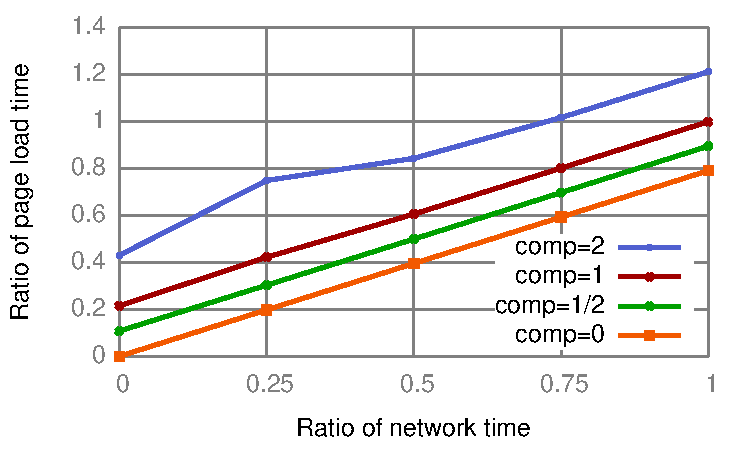
\includegraphics[width=3in]{../graphs/whatif/ilivid.pdf}
    \caption[]{\label{fig:whatif} Median reduction in PLT
    for torchbrowser.com when hypothetical computation and network speeds are varied.}
\end{figure}

{\bf Fitting $K$.}

% TODO(cs): show off some predictions we can make with this model.
